% Chapter 2

\chapter{Background} % Main chapter title

\label{Chapter2} % Change X to a consecutive number; for referencing this chapter elsewhere, use \ref{ChapterX}

%----------------------------------------------------------------------------------------
%	SECTION 1
%----------------------------------------------------------------------------------------

\section{Newton's Method} \label{Sect:Newton'sMethod}
Overview of why we would use Newton's method??

 Newton's method is an iterative method used to find solutions to functions. The needed input to the method are the function, written so that it is equal to zero, a value to indicate how exact the solution needs to be, and an initial guess. Other useful inputs include a maximum number of iterations as well a tolerance for how far off the initial guess is. Consider the system of functions
\begin{eqnarray}
 \begin{cases}
  f_1(x_1,x_2, \dots,x_m)&=f_1(\mathbf{x}) =0\\
  f_2(x_1,x_2, \dots,x_m)&=f_2(\mathbf{x}) =0\\
  &\vdots\\
  f_n(x_1,x_2, \dots,x_m)&=f_n(\mathbf{x}) =0.\\
 \end{cases}
\end{eqnarray}
Suppose you have an initial guess $\mathbf{x_0}$. Newton's method involves moving along linear approximations to try and find the zeros, or in this case, the solution to the system. To do this, start by plugging in the guess into the system, the values obtained are called the residual,
\begin{eqnarray}
 \begin{bmatrix}
 f_1(\mathbf{x_0})\\
 f_2(\mathbf{x_0})\\
 \vdots \\
 f_n(\mathbf{x_0})
 \end{bmatrix} 
 =
 \begin{bmatrix}
 r_1\\
 r_2 \\
 \vdots\\
 r_n
 \end{bmatrix}
 =\mathbf{R}.
\end{eqnarray}
Next, check the size of the residual $\mathbf{R}$ by taking the norm. For this paper, the norm will be specified in each case and will either be the infinity norm or the grid two norm. If the norm of $\mathbf{R}$ is less than the specified value for accuracy, then the initial guess is accepted as the solution. If not, then the norm can be checked to be within a specified tolerance. This helps insure that Newton's method has a reasonable chance of converging. If the norm of the residual is less than the specified value for tolerance, then a new guess is calculated. The way a new guess is calculated, is using the derivative, in this case the Jacobian. 


%-----------------------------------
%	SUBSECTION 1
%-----------------------------------
\subsection{Newton's Method in One Dimension}

First consider the case where $n=1$ and $m=1$. Then the linear approximation for $f(x)$ is
\begin{eqnarray}
 f(x) \approx f(x_0) + f'(x_0)(x-x_0).
\end{eqnarray}
Now since we are solving for a zero of $f$ we want to know the $x$ such that $f(x)=0$. Call this $x$ that we are solving for $x_1$, for now. The next step is to set $f(x_1) =0$ and try and solve for $x_1$, giving
\begin{eqnarray} \label{eqn:newtonlinear}
f(x_0) \approx f'(x_0)(x_0-x_1).
\end{eqnarray}
We can know $f(x_0)$ and $f'(x_0)$ so we can solve for $s = x_0-x$ then our next guess will become $x_1 = x_0-s = x_0-x_0+x=x$. With this linear approximation $f(x_1) \approx 0$ however another iteration can be made using $x_1$ as the guess and solving for $x_2$ to check this. In other works $x_1$ becomes our new guess so we begin again by calculating the residual, then the norm of the residual and so on. This process continues until either, (1) the residual's norm is less than the specified accuracy value or, (2) the specified maximum number of iterations is met, or (3) Occasionally, the Jacobian will lead to a guess that can lead to the residual having a norm that is greater than the tolerance. In any of these three cases the Newton iterations cease. In case one, the current iteration's guess, $x_i$, becomes the numerical estimate from the solution. In the other two cases and error message occurs. 

%-----------------------------------
%	SUBSECTION 2
%-----------------------------------

\subsection{Newton's Method in Multiple Dimensions}


Now translating this to multiple dimension, $f'(x)$ is now the Jacobian of $f$
\begin{eqnarray}
J_f = \begin{bmatrix}
\pd{}{f_1}{x_1} & \cdots & \pd{}{f_1}{x_m} \\
\vdots & \ddots & \vdots \\
\pd{}{f_n}{x_1} & \cdots & \pd{}{f_n}{x_m}.
\end{bmatrix}
\end{eqnarray}
Equation (\ref{eqn:newtonlinear}) becomes 
\begin{eqnarray}
J_f(\mathbf{x_0})s \approx f(\mathbf{x_0}) = \mathbf{R}
\end{eqnarray}
where $s = \mathbf{x_0} - \mathbf{x_1}$. In Matlab this system can be solve by using the build in $\backslash$ command. Thus $s = J_f(\mathbf{x_0})\backslash \mathbf{R}$. Then the same process as for the one dimensional case continues. 

%----------------------------------------------------------------------------------------
%	SECTION 2
%----------------------------------------------------------------------------------------

\section{Splitting Method ODE} \label{Sect:Splitting}

% CODE: odeplay3v5.m, odeplay3v2$\_$plot.m \\
% REFERENCES: ``An Unconditionally Stable One-Step Scheme for Gradient Systems", David J. Eyre \cite{Eyre} \\
The main goal of this section is to look at discretization of gradient flows using Eyre's paper \parencite{Eyre}.  This section will start with a basic overview of the Eyre paper then look at an example discussed in the paper and compare numerical methods used for the example. 

``An Unconditionally Stable One-Step Scheme for Gradient Systems" presents a numerical method for solving the ODE, 
\begin{eqnarray}
\frac{du}{dt} = - \grad F(u), \quad u(0)=u_0
\end{eqnarray}
using convexity splitting. The basic idea is to set up a scheme that splits each time step based on convexity. Though the paper mostly discusses results for ODEs, the method is applicable to gradient flow PDEs. One example of the application to PDE is included but the ODE example is closer to the equations that will be used for the Stefan problem. 

To take a closer look at example on page 9 of \cite{Eyre}, which discusses a scheme that splits 
%
\begin{eqnarray} \label{ODEexample}
f(u) = \frac{du}{dt} = u - u^3, 
\end{eqnarray}
%
by its contractive $f_c(u)={5}u$ and expansive $-f_e(u)=f(u)-f_c(u)={6}u-u^3$ terms, a solution was calculated with MATLAB using a few methods. The convexity splitting scheme, 
%
\begin{eqnarray} \label{equn scheme ac5}
(1+5\mytau)U^{n+1}=(1+6\mytau)U^n-\mytau(U^n)^3 
\end{eqnarray}
%
where $\mytau$ is the time step, was compared to both MATLAB ode45 and backward Euler. In tables \ref{table:erroru0n075} and \ref{table:erroru0p001} the error, calculated by taking the max of error between the respective method and the exact solution at each time step, was measured for a couple initial conditions, $u_0$. The time was run from 0 to 5. The build in MATLAB function ode45 determines a variant time step, thus ode45 was only calculated once for each initial condition. A couple other initial conditions were tried with very similar results. 

\mpcomment{Explain what is $u0$? Are you reporting on the errors? is $\#$ the size of time step? perhaps explain overall every part of the table}

\mpcomment{Lisa's question: why is the error bigger for splitting scheme than in BE? MP suggestion: use LTE analysis to find out?}

\mpcomment{Computational effort?}

\begin{table}[H]                               
\centering                                     
\begin{tabular}{|c|c|c|c|c|c||c|} 
\hline                                        
$u_0$ & time steps & Backward Euler Error & $\alpha_{BE}$ & Splitting Scheme Error & $\alpha_{SS}$ & ode45 error \\
\hline                                         
-0.75 & 10 & 0.0245122 & - & 0.1127655 & - & \multirow{5}{*}{0.0000390 } \\      
\hhline{------~}                          
-0.75 & 100 & 0.0029494 & 0.920 & 0.0207292 & 0.736 &  \\       
\hhline{------~}                                            
-0.75 & 1000 & 0.0003011 & 0.991 & 0.0022693 & 0.961 & \\      
\hhline{------~}                                         
-0.75 & 10000 & 0.0000302 & 0.999 & 0.0002291 & 0.996 &  \\     
\hhline{------~}                                         
-0.75 & 100000 & 0.0000030 & 1.000 & 0.0000229 & 1.000 &  \\   
\hline                                          
\end{tabular}                                 
\caption{Max error over time for initial condition $u_0=-0.75$ for equation~\eqref{ODEexample} at $t=T=5$.}                   \label{table:erroru0n075}                                 
\end{table}    

\begin{table}[H]                                
\centering                                    
\begin{tabular}{|c|c|c|c|c|c||c|}               
\hline                                             
$u_0$ & time steps & Backward Euler Error & $\alpha_{BE}$ & Splitting Scheme Error & $\alpha_{SS}$ & ode45 error \\
\hline                                                
0.01 & 10 & 0.3418509 & - & 0.7913338 & - & \multirow{5}{*}{0.0000158} \\    
\hhline{------~}                                       
0.01 & 100 & 0.0352905 & 0.986 & 0.3770012 & 0.322 & \\         
\hhline{------~}                                               
0.01 & 1000 & 0.0035146 & 1.002 & 0.0446279 & 0.927 & \\       
\hhline{------~}                                      
0.01 & 10000 & 0.0003513 & 1.000 & 0.0045159 & 0.995 &  \\     
\hhline{------~}                   
0.01 & 100000 & 0.0000351 & 1.000 & 0.0004521 & 1.000 &  \\     
\hline                                         
\end{tabular}                                                   \caption{Max error over time for initial condition $u_0=0.01$ for equation~\eqref{ODEexample} at $t=T=5$.}               \label{table:erroru0p001}            
\end{table}   



		\begin{figure}[H]
		\centering
		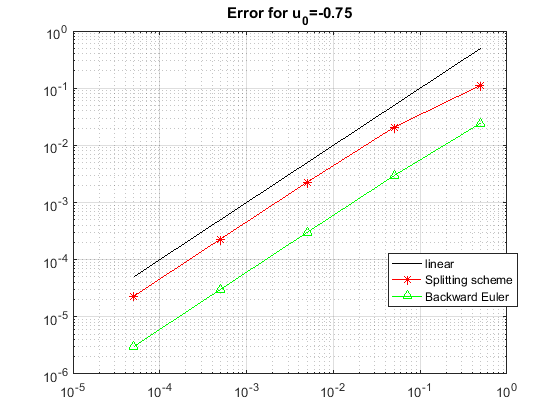
\includegraphics[width=.4\textwidth]{odeplayerrorn075.png}
        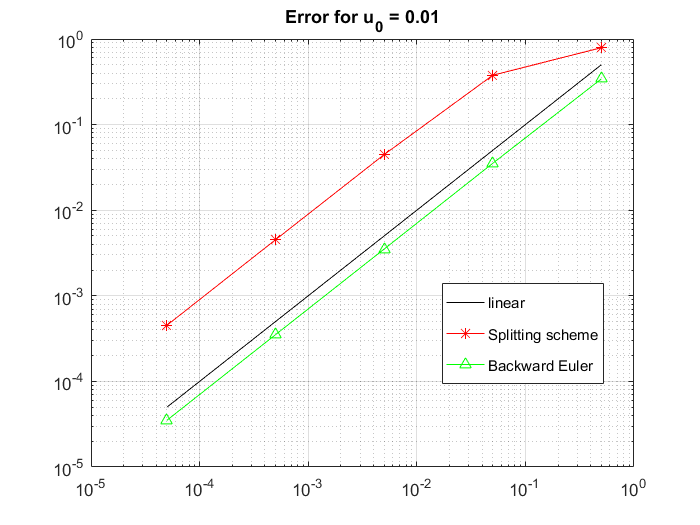
\includegraphics[width=.4\textwidth]{odeplayerror001.png}
		\caption{Error plots for backward Euler and the splitting scheme on loglog graphs. \mpcomment{Define what error means}}
		\label{fig:odeplayerror}
		\end{figure}



